\documentclass[tikz, border=5mm]{standalone}
\usepackage[T1]{fontenc}
\usepackage{mathpazo}
\usepackage[scaled]{beramono}
\usetikzlibrary{positioning}

\begin{document}
	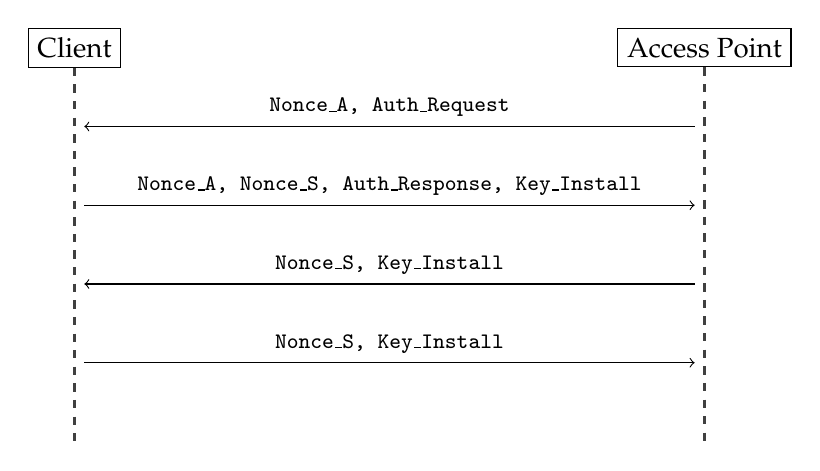
\begin{tikzpicture}[node distance=1cm, on grid, font=\footnotesize]
		
		%\draw[help lines] (-2,0) grid (2,-10);
		
		\tikzstyle{timeLine} = [darkgray,dashed,thick]
		
		% Nodes
		\node[draw, rectangle, font=\normalsize] (client) at (-4,0) {Client};
		\node[draw, rectangle, font=\normalsize] (ap) at (4,0) {Access Point};
		
		% Timelines
		\draw[timeLine] (client) -- ++(0,-5);
		\draw[timeLine] (ap) -- ++(0,-5);
		
		% Messages
		\node[below=of client] (m1_client) {};
		\node[below=of ap] (m1_ap) {};
		\draw[->] (m1_ap) -- node[above] {\texttt{Nonce\_A, Auth\_Request}} (m1_client);
		
		\node[below=of m1_client] (m2_client) {};
		\node[below=of m1_ap] (m2_ap) {};
		\draw[->] (m2_client) -- node[above] {\texttt{Nonce\_A, Nonce\_S, Auth\_Response, Key\_Install}} (m2_ap);
		
		\node[below=of m2_client] (m3_client) {};
		\node[below=of m2_ap] (m3_ap) {};
		\draw[->] (m3_ap) -- node[above]{\texttt{Nonce\_S, Key\_Install}} (m3_client);
		
		\node[below=of m3_client] (m4_client) {};
		\node[below=of m3_ap] (m4_ap) {};
		\draw[->] (m4_client) -- node[above]{\texttt{Nonce\_S, Key\_Install}} (m4_ap);
		%\draw[->] (ap) -- node[below] {\texttt{ACK}} (client);
		
	\end{tikzpicture}
\end{document}
